% Coordinates and normalisation, v1 (D-129 follow-up).
% Third figure in the set. jan-blockscheme-v4 = model topology; training-objective-v1 =
% the training problem in time; this one = where the numbers live.
% Answers two questions the other two cannot: where the velocity states come from, and how a
% data-derived normalisation is wrapped around exact SI physics without touching it.
% Notation follows v4 and the code: x = normalised state, x^phys = SI, xtilde/xbar = the
% physical/augmented partition, code names in typewriter so data.py can be read against it.
% Style: docs/writeup/figure-style.md.
% Compile: pdflatex coordinates-normalisation-v1.tex
\documentclass[border=12pt]{standalone}
\usepackage{tikz}
\usetikzlibrary{arrows.meta, calc, decorations.pathreplacing}
\usepackage{amsmath}

\begin{document}
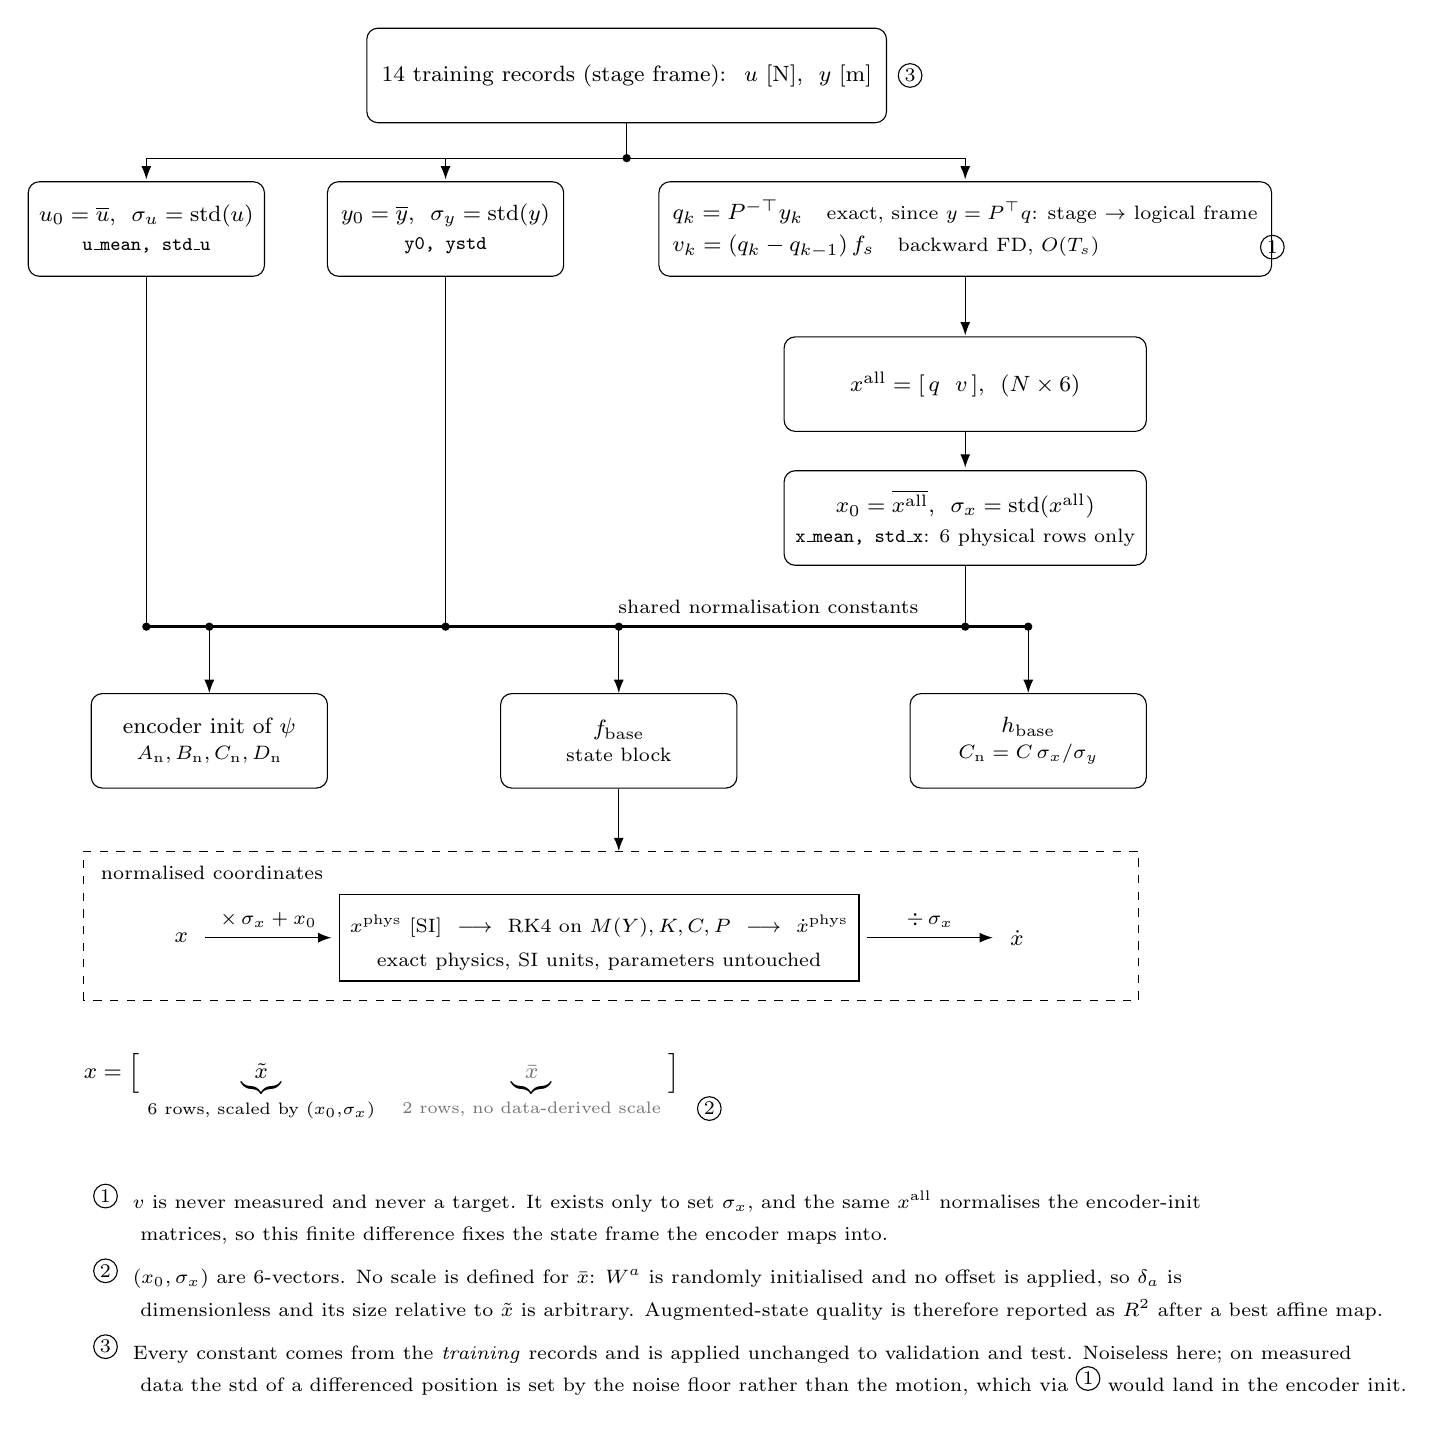
\begin{tikzpicture}[>=Latex, font=\footnotesize,
  block/.style={draw, rounded corners, minimum width=30mm, minimum height=12mm, align=center},
  wide/.style={draw, rounded corners, minimum height=12mm, align=left, inner sep=5pt},
  ann/.style={font=\scriptsize, align=left},
  anc/.style={font=\scriptsize, align=center},
  grey/.style={black!55},
  jn/.style={circle, fill, minimum size=3pt, inner sep=0pt},
  cal/.style={draw, circle, inner sep=0.9pt, font=\scriptsize}]

%% ===================== source =====================
\node[wide, minimum width=66mm, align=center] (data) at (7.8,0)
  {14 training records (stage frame): \ $u$ [N], \ $y$ [m]};
\node[cal] (c3) at (11.4,0) {3};

%% distribution bar
\draw (data.south) -- (7.8,-1.05);
\draw (1.7,-1.05) -- (12.1,-1.05);
\node[jn] at (7.8,-1.05) {};
\draw[->] (1.7,-1.05)  -- (1.7,-1.32);
\draw[->] (5.5,-1.05)  -- (5.5,-1.32);
\draw[->] (12.1,-1.05) -- (12.1,-1.32);

%% ===================== three derivations =====================
\node[block] (nu) at (1.7,-1.95)
  {$u_0=\overline{u}$, \ $\sigma_u=\mathrm{std}(u)$\\[1pt]{\scriptsize\texttt{u\_mean, std\_u}}};
\node[block] (ny) at (5.5,-1.95)
  {$y_0=\overline{y}$, \ $\sigma_y=\mathrm{std}(y)$\\[1pt]{\scriptsize\texttt{y0, ystd}}};
\node[wide, minimum width=68mm] (nx) at (12.1,-1.95)
  {$q_k=P^{-\top}y_k$ \ \ {\scriptsize exact, since $y=P^{\top}q$: stage $\to$ logical frame}\\[2pt]
   $v_k=(q_k-q_{k-1})\,f_s$ \ \ {\scriptsize backward FD, $O(T_s)$}};
\node[cal] (c1) at (16.0,-2.18) {1};

\draw[->] (nx.south) -- (12.1,-3.30);
\node[block, minimum width=46mm] (xall) at (12.1,-3.92)
  {$x^{\mathrm{all}}=[\,q \ \ v\,]$, \ $(N \times 6)$};
\draw[->] (xall.south) -- (12.1,-4.98);
\node[block, minimum width=46mm] (cx) at (12.1,-5.62)
  {$x_0=\overline{x^{\mathrm{all}}}$, \ $\sigma_x=\mathrm{std}(x^{\mathrm{all}})$\\[1pt]
   {\scriptsize\texttt{x\_mean, std\_x}: 6 physical rows only}};

%% ===================== shared constants bus =====================
\draw (nu.south) -- (1.7,-7.00);
\draw (ny.south) -- (5.5,-7.00);
\draw (cx.south) -- (12.1,-7.00);
\draw[line width=1.3pt] (1.7,-7.00) -- (12.9,-7.00);
\foreach \x in {1.7,2.5,5.5,7.7,12.1,12.9}{\node[jn] at (\x,-7.00) {};}
\node[anc, anchor=south, inner sep=3pt] at (9.6,-6.94) {shared normalisation constants};

%% ===================== three consumers =====================
% NB: subscript n (not a bar) for normalised matrices. v4 already uses a bar for the
% augmented partition xbar, and reusing it here would give the bar two meanings.
\node[block] (enc) at (2.5,-8.45)
  {encoder init of $\psi$\\{\scriptsize $A_{\mathrm{n}},B_{\mathrm{n}},C_{\mathrm{n}},D_{\mathrm{n}}$}};
\node[block] (fb)  at (7.7,-8.45) {$f_{\mathrm{base}}$\\{\scriptsize state block}};
\node[block] (hb)  at (12.9,-8.45)
  {$h_{\mathrm{base}}$\\{\scriptsize $C_{\mathrm{n}}=C\,\sigma_x/\sigma_y$}};
\draw[->] (2.5,-7.00)  -- (enc.north);
\draw[->] (7.7,-7.00)  -- (fb.north);
\draw[->] (12.9,-7.00) -- (hb.north);

%% ===================== inside f_base =====================
\draw[dashed] (0.9,-11.75) rectangle (14.3,-9.85);
\node[ann, anchor=north west] at (1.0,-9.92) {normalised coordinates};
\draw[->] (fb.south) -- (7.7,-9.85);

\node[anchor=east] at (2.35,-10.95) {$x$};
\draw[->] (2.45,-10.95) -- (4.05,-10.95);
\node[anc, anchor=south, inner sep=2pt] at (3.25,-10.90) {$\times\,\sigma_x + x_0$};

\draw (4.15,-11.50) rectangle (10.75,-10.40);
\node[anc] at (7.45,-10.80)
  {$x^{\mathrm{phys}}$ [SI] \ $\longrightarrow$ \ RK4 on $M(Y),K,C,P$ \ $\longrightarrow$ \ $\dot x^{\mathrm{phys}}$};
% black, not grey: this is the claim of the figure, and grey is reserved for
% "present but explicitly not part of the claim" (figure-style.md S2).
\node[anc] at (7.45,-11.26) {exact physics, SI units, parameters untouched};

\draw[->] (10.85,-10.95) -- (12.45,-10.95);
\node[anc, anchor=south, inner sep=2pt] at (11.65,-10.90) {$\div\,\sigma_x$};
\node[anchor=west] at (12.55,-10.95) {$\dot x$};

%% ===================== the partition =====================
\node[anchor=west, inner sep=0pt] at (0.9,-12.85)
  {$x=\Big[\,
    \underbrace{\tilde x}_{\text{6 rows, scaled by }(x_0,\sigma_x)} \ \ \
    \underbrace{{\color{black!55}\bar x}}_{{\color{black!55}\text{2 rows, no data-derived scale}}}
    \,\Big]$};
\node[cal] (c2) at (8.85,-13.12) {2};

%% ===================== callouts =====================
\node[ann, anchor=north west] at (0.9,-13.95)
  {\raisebox{0.2pt}{\tikz\node[cal]{1};} \ $v$ is never measured and never a target. It exists
   only to set $\sigma_x$, and the same $x^{\mathrm{all}}$ normalises the encoder-init\\
   \phantom{\raisebox{0.2pt}{\tikz\node[cal]{1};} \ } matrices, so this finite difference
   fixes the state frame the encoder maps into.\\[4pt]
   \raisebox{0.2pt}{\tikz\node[cal]{2};} \ $(x_0,\sigma_x)$ are 6-vectors. No scale is defined
   for $\bar x$: $W^a$ is randomly initialised and no offset is applied, so $\delta_a$ is\\
   \phantom{\raisebox{0.2pt}{\tikz\node[cal]{2};} \ } dimensionless and its size relative to
   $\tilde x$ is arbitrary. Augmented-state quality is therefore reported as $R^2$ after a
   best affine map.\\[4pt]
   \raisebox{0.2pt}{\tikz\node[cal]{3};} \ Every constant comes from the \emph{training}
   records and is applied unchanged to validation and test. Noiseless here; on measured\\
   \phantom{\raisebox{0.2pt}{\tikz\node[cal]{3};} \ } data the std of a differenced position
   is set by the noise floor rather than the motion, which via \raisebox{0.2pt}{\tikz\node[cal]{1};}
   would land in the encoder init.};

\end{tikzpicture}
\end{document}

% ---------------------------------------------------------------------------
% SUGGESTED CAPTION
%
% Coordinates and normalisation. All normalisation constants are estimated from the 14
% training records. The input and output constants are ordinary sample statistics; the state
% constants are taken from a data proxy for the state, built by mapping the measured stage
% positions into the logical frame (exact, since y = P^T q) and differencing them once for
% velocity. That proxy is the only place velocities are constructed in the training path.
% One shared set of constants feeds all three consumers: the encoder initialisation, the
% baseline state block, and the normalised output matrix. Inside the state block the
% normalisation is undone, the physical ODE is integrated in SI units with the parameters
% untouched, and the derivative is rescaled, so normalisation is a conditioning transform
% wrapped around exact physics rather than a change to it. Callouts mark the three places
% where the data-derived scaling and the model do not line up.
% ---------------------------------------------------------------------------
